\documentclass[10pt,a4paper]{article}
\usepackage[utf8]{inputenc}
\usepackage[english]{babel}
\usepackage{amsmath}
\usepackage{amsfonts}
\usepackage{amssymb}
\usepackage{graphicx}
\author{Gérard Tio Nogueras}
\title{COMP6224: Foundation of Cyber Security}
\begin{document}
\maketitle
\newpage
\tableofcontents
\newpage
\section{I<ntroduction}
Teacher: : Vladimiro Sassone\\
"People are the weakest node in network and systems"
\subsection{what is cyber security?}
Very important to make risk management:\\
"How much spend to defend, depending on the risk and power of the possible attacker on given target"\\ \\
Some definitions:\\
\textbf{Cyber security}: protection of the cyberspace against cyber threats and vulnerabilities.\\
\textbf{Cyber space}: complex of activities carried out through networks of computers.\\
\textbf{Cyber threat}: typical threats include unauthorised access, destruction, system overrun and takeover, propagation of malicious code, data thieving and fabrication, ...\\
\textbf{Cyber vulnerability}:  the presence of weaknesses or loopholes in systems which may lead (systematically) to cyber attacks. \\
\textbf{National security}: attacks to critical infrastructures such as Transport, Energy and  Communications can have devastating effects, and are now regular part of warfare and terrorist scenarios.\\
\textbf{Gvt and public bodies}: the robustness to intrusion and tamper of electronic services, 
which typically hold very sensitive information.\\
\textbf{The economic processes}:  the protection of industrial secrets and practices, the confidentiality of 
business information and tenders; the viability of the network economy, just think of the banking system. \\
\textbf{The citizen}: the privacy and legitimate use of personal data against de-anonymisation and 
impersonation attacks from all sources; the challenged from cybercrime.\\
\subsection{Challenges ?}
To create a strong learning and teaching programme to limit threats and vuln.\\
\subsection{Unfair ?}
Because even if the computers are maintained by the smartest people, they can't prevent the user's mistakes.
\subsection{What is needed ?}
Education
\subsection{Numbers}
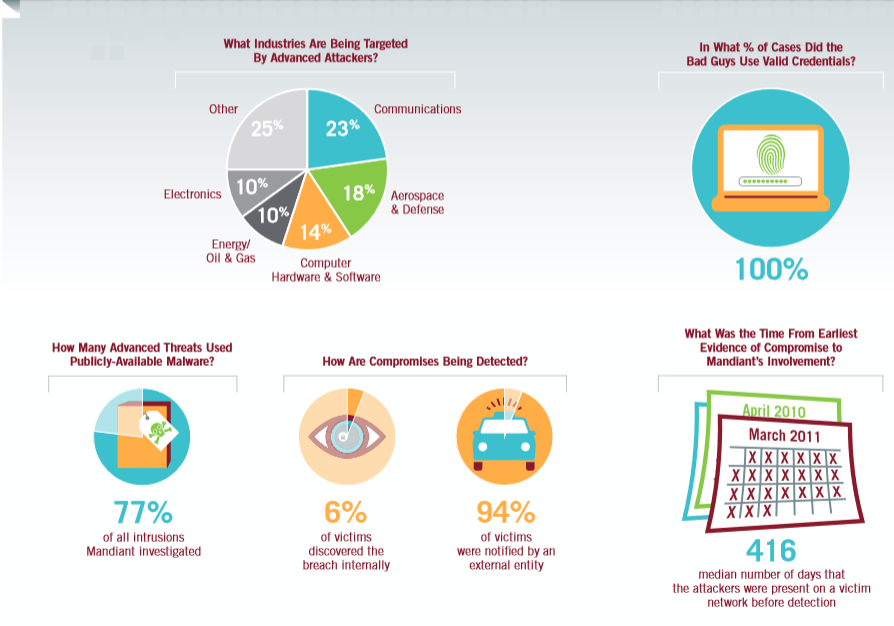
\includegraphics[scale=0.55]{1_numbers.png}\\

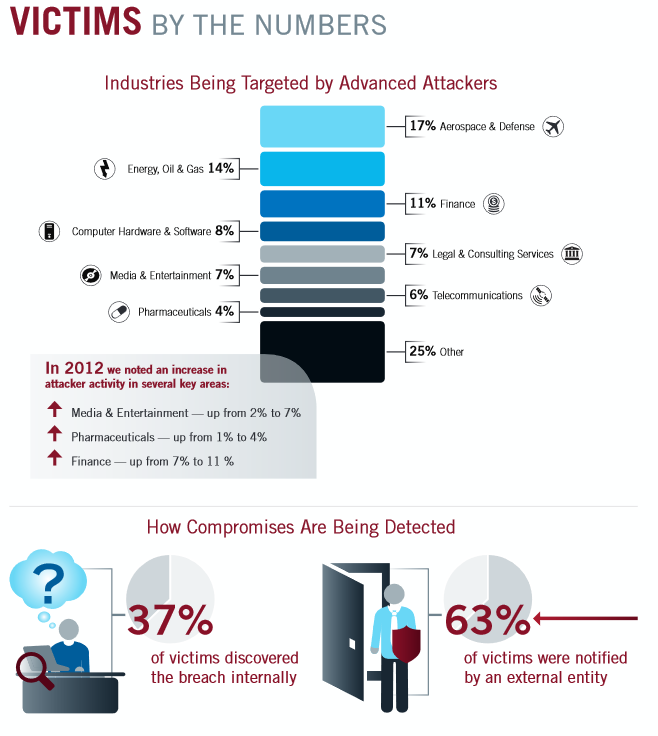
\includegraphics[scale=0.55]{2_numbers.png}\\

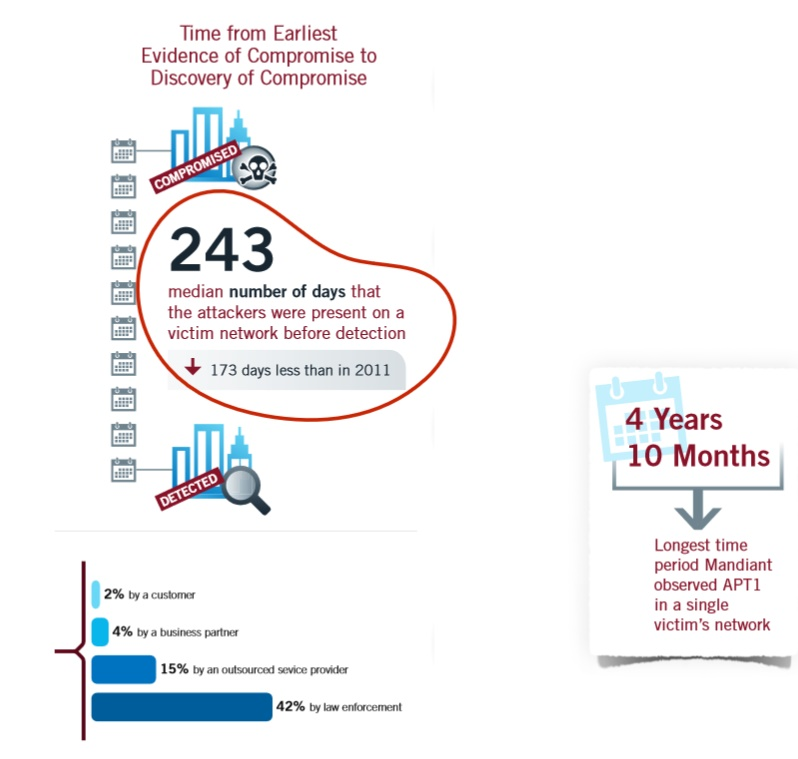
\includegraphics[scale=0.55]{3_numbers.png}
\subsection{Malware is only half of the story}
Malware explain half of what happend, but you still have to analyse and research the registry entries, event logs, scheduled tasks logs, inventory mgnt logs, network traffic capture and finaly file system artifacts.
\subsection{Old is the new door}
Backdoors were used as backdoors to be resilient against detection and remote access.\\ Lately these backdoors became passive backdoors meaning that they don't generate any network traffic and are harder to detect. They don't generate traffic work. Here are 2 example of passive backdoors:\\
\textbf{Port Listeners}: 

\end{document}